\documentclass{article}

\usepackage{xstring}
\usepackage{fancyhdr}
\usepackage{extramarks}
\usepackage[plain]{algorithm}
\usepackage{algpseudocode}
\usepackage{parskip}
\usepackage{enumerate}
\usepackage{setspace}
\usepackage{subfig}
\usepackage{listings}
\usepackage{pgfplots}
\usepackage{url}
\usepackage[hidelinks]{hyperref}
\usepackage{color}
\usepackage{courier}
\usepackage{hyperref}
\usepackage{graphicx}

%
% Basic Document Settings
%
\graphicspath{ {images/} }

\topmargin=-0.45in
\evensidemargin=0in
\oddsidemargin=0in
\textwidth=6.5in
\textheight=9.0in
\headsep=0.25in

\linespread{1.1}

\pagestyle{fancy}
\lhead{CreateGraphics Tutorial}
\rhead{Grace}
\lfoot{\lastxmark}
\cfoot{\thepage}

\renewcommand\headrulewidth{0.4pt}
\renewcommand\footrulewidth{0.4pt}

\setlength\parindent{0pt}

\definecolor{dkgreen}{rgb}{0,0.6,0}
\definecolor{gray}{rgb}{0.5,0.5,0.5}
\definecolor{mauve}{rgb}{0.58,0,0.82}

\lstset{frame=tb,
  language=Java,
  aboveskip=3mm,
  belowskip=3mm,
  showstringspaces=false,
  columns=flexible,
  basicstyle={\small\ttfamily},
  numbers=none,
  numberstyle=\tiny\color{gray},
  keywordstyle=\color{blue},
  commentstyle=\color{dkgreen},
  stringstyle=\color{mauve},
  breaklines=true,
  breakatwhitespace=true,
  tabsize=3
}

\begin{document}

\section{Introduction}
The CreateGraphics package allows the developer to:

\begin{itemize}
\item Generate basic graphics
\item Add event listeners
\item Sound functionality for built-in mp3 files
\end{itemize}

Functionality is performed using the createjs javascript library available at:\\
\url{http://www.createjs.com/}. 

\section{Graphics}
In order to work with the CreateGraphics package, you need to include the 
following line at the top of your Grace file:

\texttt{import createGraphics as cg}

The graphics object needs to be created with the following command:

\texttt{def graphics = createGraphics(width,height)} 

where width and height correspond to the desired graphics window width
and height. For example:

\begin{lstlisting}
def width = 300
def height = 300
def graphics = cg.createGraphics(width, height)
\end{lstlisting}

\section{Shapes}
The following shape objects are available in CreateGraphics:Circle, Rectangle, Rounded Rectangle, PolyStar, Ellipse, Text, Line, and Custom Shape.
To draw one of these objects to the screen, pass a message to the graphics object:

\begin{itemize}
\item addCircle
\item addRect
\item addPolyStar
\item addRoundRect
\item addEllipse
\item addText
\item addLine
\item addCustomShape
\end{itemize}

For instance, to add a circle to the window, you might do the following:
\begin{lstlisting}
import createGraphics as cg
def graphics = cg.createGraphics(300, 300)
def circle = graphics.addCircle
circle.draw
\end{lstlisting}
Each shape has different parameters that are used to create it. These parameters have default values, so you don't need to set each
one every time you create an shape.

\subsection{Common Parameters}
There are a few parameters that are common to each type of shape.

\begin{itemize}
\item \textbf{location} (Point): The x,y coordinates where the shape will be placed in the graphics window. Coordinates are expressed in Grace "Point" notation: x@y. Keep in mind that the origin is in the upper left corner of the window, so 10@10 will be 10 down and 10 right from the corner of the window.
\item \textbf{color} (String): The color of the shape. Most basic colors can be set as "red", "blue", etc. However, you can also use 6-digit hex numbers 
such as "\#CC3300" that corresponds to an HTML 5 hex colors. See \url{http://www.w3schools.com/tags/ref_colorpicker.asp} for more details.
\item \textbf{fill} (Boolean): Whether or not you want to fill in the shape when it is drawn on the window.
\end{itemize}

\textbf{Chaining} \\
In order to make the resulting code more compact, CreateGraphics has a number of "chaining"
methods that you can use instead of setting parameters individually. The common ones are:
\begin{itemize}
\item on(location)
\item colored(color)
\item filled(fill)
\end{itemize}

This allows you to construct the object like this:

\begin{lstlisting}
import createGraphics as cg
def graphics = cg.createGraphics(300, 300)
graphics.addCircle.colored("red").filled(true).draw
\end{lstlisting}

\subsection{Circle}
\textbf{Create:} graphics.addCircle

Parameters:
\begin{itemize}
\item \textbf{radius} (Number): The length of the circle radius
\end{itemize}

Chaining Methods:
\begin{itemize}
\item \textbf{setRadius(Number)}
\end{itemize}

\subsection{Rectangle}
\textbf{Create:} graphics.addRect

Parameters:
\begin{itemize}
\item \textbf{width} (Number): Width of the rectangle
\item \textbf{height}(Number): Height of the rectangle
\end{itemize}

Chaining Methods:
\begin{itemize}
\item \textbf{setWidth(Number)} 
\item \textbf{setHeight(Number)}
\end{itemize}

\subsection{Rounded Rectangle}
\textbf{Create:} graphics.addRoundRect

Parameters:
\begin{itemize}
\item \textbf{width} (Number): Width of the rectangle
\item \textbf{height}(Number): Height of the rectangle
\item \textbf{radius} (Number): Radius of the rounded corners
\end{itemize}

Chaining Methods:
\begin{itemize}
\item \textbf{setWidth(Number)} 
\item \textbf{setHeight(Number)}
\item \textbf{setRadius(Number)}
\end{itemize}

\subsection{PolyStar}
\textbf{Create:} graphics.addPolyStar

Parameters:
\begin{itemize}
\item \textbf{size} (Number): Length of each side of the star
\item \textbf{sides} (Number): Number of sides
\item \textbf{pointSize} (Number): Size of the points
\item \textbf{angle} (Number): Angle between the points
\end{itemize}

Chaining Methods:
\begin{itemize}
\item \textbf{setSize(Number)} 
\item \textbf{setSides(Number)} 
\item \textbf{setPointSize(Number)} 
\item \textbf{setAngle(Number)}
\end{itemize}

\subsection{Ellipse}
\textbf{Create:} graphics.addEllipse

Parameters:
\begin{itemize}
\item \textbf{width} (Number): Width of the ellipse
\item \textbf{height}(Number): Height of the ellipse
\end{itemize}

Chaining Methods:
\begin{itemize}
\item \textbf{setWidth(Number)} 
\item \textbf{setHeight(Number)}
\end{itemize}

\subsection{Text}
\textbf{Create:} graphics.addText

Parameters:
\begin{itemize}
\item \textbf{content} (String): The content of the string
\end{itemize}

Chaining Methods:
\begin{itemize}
\item \textbf{setText(String)} 
\end{itemize}

\subsection{Line}
\textbf{Create:} graphics.addLine

Parameters:
\begin{itemize}
\item \textbf{start} (Point): Location of the starting point of the line
\item \textbf{end} (Point): Location of the ending point of the line
\end{itemize}

Chaining Methods:
Parameters:
\begin{itemize}
\item \textbf{setStart(Point)} 
\item \textbf{setEnd(Point)}
\end{itemize}

\subsection{Custom Shape}
This shape consists of a set of points that you add in order to make a custom shape.
Instead of configuring preset parameters, you just add points to the shape. 
\textbf{Create:} graphics.addCustomShape
Methods:
\begin{itemize}
\item \textbf{addPoint} (Point): Add this point to shape the object
\end{itemize}

The addPoint method returns the object, that you can chain it together. For example:
\begin{lstlisting}
import createGraphics as cg
def graphics = cg.createGraphics(300, 300)
graphics.addCustomShape.colored("red").addPoint(40@40).addPoint(0@40).addPoint(40@0).draw
\end{lstlisting}

\section{Drawing a Shape}
To draw a shape on the graphics window, first create it, then configure it, and then draw it. The following code
creates the output down in Figure \ref{fig:red_circle}.
\begin{lstlisting}
import createGraphics as cg
def graphics = cg.createGraphics(200, 200)
def circle = graphics.addCircle
circle.color := "red"
circle.radius := 20
circle.position := 30@30
circle.fill := true
circle.draw
\end{lstlisting}

\begin{figure}[h]
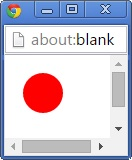
\includegraphics{red_circle}
\centering
\caption{Creating a red circle}
\label{fig:red_circle}
\end{figure}

\section{Adding a Click Handler}
Adding a click handler to a shape defines a block of code that will be executed when the shape is clicked. For instance,
let's say that we want the red circle to turn blue when it is clicked, and we want to add a message to the user. 
Then you would add something like this:
\begin{lstlisting}
import createGraphics as cg
def graphics = cg.createGraphics(200, 200)
def circle = graphics.addCircle
circle.color := "red"
circle.click := { 
  print("clicked circle") 
  circle.color := "blue"
  circle.draw
}
circle.draw
\end{lstlisting}
The \color{blue} circle.draw \color{black} line located in the click block is used to update the circle object after its color
has been changed. The line \color{blue}circle.color := ``blue'' \color{black} updates the variable inside the circle object, but
a message to circle.draw needs to be sent in order for the graphics to actually be updated.

\section{Adding sound}
CreateGraphics supports basic sounds. All sounds are preloaded in the browser and cannot be customized at this time.
To play a sound, just use the "play" method of the graphics object. For example:
\begin{lstlisting}
import createGraphics as cg
def graphics = cg.createGraphics(200, 200)
def circle = graphics.addCircle
circle.color := "red"
circle.click := { 
  print("clicked circle") 
  graphics.play("bicycle_bell")
  circle.draw
}
circle.draw
\end{lstlisting}


The following sounds are available: note1, note2, note3, note4, note5, note6, note7, note8, bicycle\_bell, snap, 
whoosh, shutter.
\end{document}
